\section{An\'alise da amostra}
\label{sec:analise}
%Fazer um estudo descritivo dos dados (gráficos e medidas). Verificar normalidade dos dados e potenciais pontos aberrantes

Nesta seção, nós apresentamos um estudo descritivo dos dados da amostra. Nesse contexto, mostramos alguns gráficos gerados por meio da linguagem R, bem como verificamos a normalidade dos dados.

\subsection{Estudo descritivo}
\label{sec:estudo}

%falar sobre os gráficos e medidas que vamos usar
Por meio da linguagem R, nós geramos três gráficos que usamos no nosso estudo. Primeiro, usamos o Q-Q Plot. Esse gráfico permite ilustrar a normalidade dos resíduos dos dados da amostra~\cite{Wilk1968}. Segundo, usamos o gráfico Boxplot para ilustrar a mediana do tempo levado para executar os testes considerando cada uma das técnicas (TE e TG), bem como onde estão localizados 50\% dos valores mais prováveis e os valores extremos. Além disso, usamos o gráfico Dotplot para ilustrar todas as variáveis, ou seja, nós mostramos o tempo de execução que cada estudante precisou para cada feature, usando cada uma das duas técnicas.

\subsection{Normalidade dos dados}
\label{sec:normalidade}

Para demonstrar a normalidade dos resíduos dos dados da nossa amostra, nós usamos o teste de aderência Shapiro-Wilk~\cite{shapirowilk}. Ele testa a hipótese nula de que uma amostra foi proveniente de uma população com distribuição normal. Portanto, se o \emph{p-value} for menor do que o nível de significância escolhido, então a hipótese nula é rejeitada, ou seja, os dados não foram provenientes de uma população com distribuição normal. Por outro lado, se o \emph{p-value} for maior que o nível de significância, então a hipótese nula não é rejeitada e consequentemente, os dados são provenientes de uma população com distribuição normal. A seguir, nós formalizamos a hipótese desse teste:

\begin{equation}
	H_{0} : \text{A amostra provém de uma população Normal}
\end{equation}

\begin{equation}
	H_{1} : \text{A amostra não provém de uma população Normal}
\end{equation}

Nesse contexto, aplicando o teste Shapiro-Wilk, nós obtivemos um \emph{p-value} igual a 0,1456, que é maior que o nosso nível de significância 0,05. Portanto, 1 não pode ser rejeitada, o que traz evidências de que os resíduos dos dados da nossa amostra provém de uma população com distribuição normal. Além disso, esse teste é baseado na estatística W~\cite{estatisticaw}. Nós obtemos um W igual a 0,9546, o que é maior que o valor 0,935 dado na tabela com os valores críticos da estatística W. Desse modo, o nosso W sendo maior que o W fornecido pela tabela\footnote{Tabela pode ser obtida em: https://github.com/rcaa/ProjetoEstatistica2013/blob/master/images/shapiro-wilk.pdf}, temos fortes evidências de normalidade dos resíduos dos dados da nossa amostra.

Esse teste de aderência pode ser interpretado por um gráfico Quantile-Quantile Plot ou Q-Q Plot. Esse gráfico ilustra se os resíduos dos dados de uma amostra provêm de uma população com distribuição normal. Além disso, ele exibe os \emph{quantiles} da amostra contra os \emph{quantiles} teóricos~\cite{Wilk1968}. Com isso, é possível visualizar a aderência dos resíduos dos dados à Normal. Na Figura~\ref{fig:grafico1}, nós ilustramos a nossa análise. A reta que cruza o gráfico representa a Normal. Percebe-se que os nossos dados estão muito próximos dessa reta, com exceção somente de 4 dos 36 pontos. Portanto, o gráfico Q-Q Plot também confirma que nossa amostra é Normal.

% EXPLICAR OS PONTOS ABERRANTES

\begin{figure*}[t]
	\caption{Q-Q Plot}
    \centering
    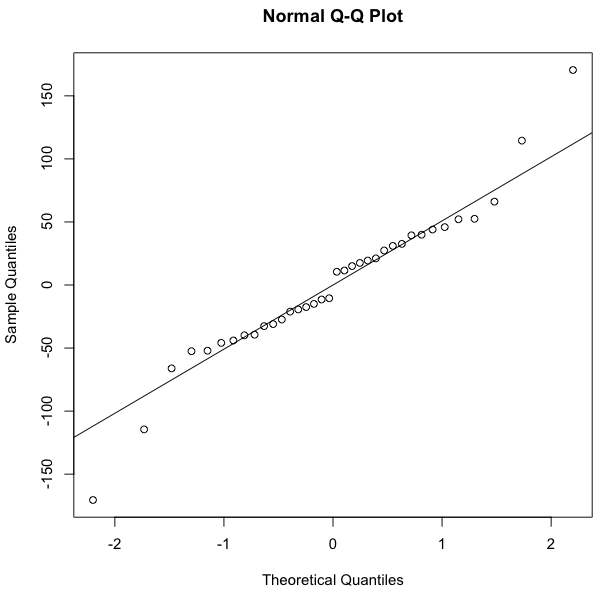
\includegraphics[width=0.4\textwidth]{images/qqplot.png}
    \caption{}
    \label{fig:grafico1}
\end{figure*}